\chapter{Corrosión y protección}\label{ch:b2:corrosion}

Déjese una gota de agua salada sobre una pieza de acero limpia. Al cabo de un día el metal está
picado en el centro de la gota, mientras que el óxido se ha formado en un anillo cerca de su
borde, donde se disuelve el oxígeno del aire. El hierro se disuelve donde hay
menos oxígeno, y el oxígeno se reduce donde hay más: la gota
es una pila que nadie ha construido, cortocircuitada a través del propio metal. Este
capítulo lee la corrosión en las \omterm{def:b2:current-potential-curves:ie-curve}{curvas intensidad--potencial}, explica por qué una
chapa galvanizada rayada no se oxida mientras que una lata de hojalata rayada sí, y
diseña la protección de un oleoducto enterrado.

\begin{recall}
El volumen del primer año: diagramas E--pH de los metales y sus dominios de inmunidad,
corrosión y \omterm{def:b2:corrosion:passivation}{pasivación} (``que una capa proteja o no es una cuestión cinética'').
\Cref{ch:b2:current-potential-curves}: \omterm{def:b2:current-potential-curves:ie-curve}{curvas intensidad--potencial}, \omterm{def:b2:current-potential-curves:limiting-current}{corrientes
límite}. \Cref{ch:b2:batteries-electrolysis}: el \omterm{def:b2:batteries-electrolysis:mixed-potential}{potencial mixto}. El volumen
escolar: corrosión, herrumbre, galvanizado.
\end{recall}

\begin{omfigure}
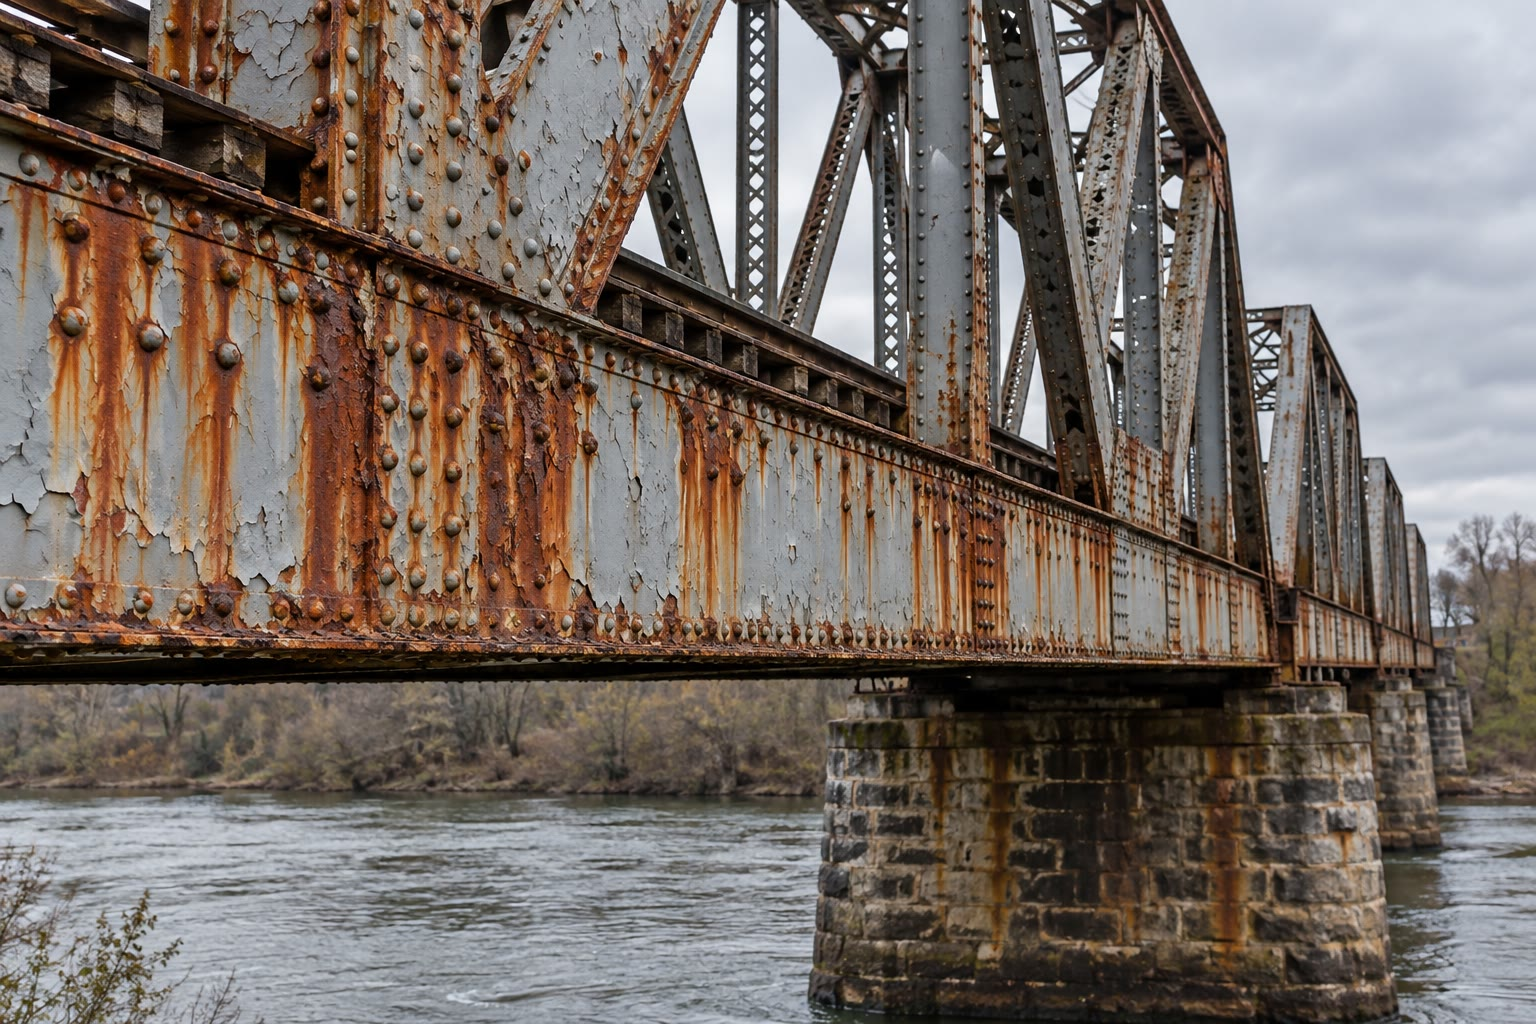
\includegraphics[width=0.62\linewidth]{images/book3/ai/b2-12-rusty-bridge.jpg}

{\small Un viejo puente ferroviario remachado. Los regueros de óxido bajan desde los remaches
y las juntas, donde el agua y el oxígeno permanecen más tiempo y la pintura falla
primero.}
\end{omfigure}

\section{La corrosión húmeda como pila en cortocircuito}

En agua con oxígeno disuelto, el hierro se oxida, \ce{Fe -> Fe^2+ + 2e-},
y los electrones son captados en la misma pieza de metal por la reducción del
dioxígeno, \ce{O2 + 2H2O + 4e- -> 4OH-} (en medio ácido, también por \ce{2H+ + 2e- -> H2}). Los
iones hierro(II) y los iones hidróxido se encuentran en el agua, y una oxidación posterior por
el aire convierte su precipitado en herrumbre, un óxido de hierro(III) hidratado.

\begin{definition}[Corrosión uniforme]\label{def:b2:corrosion:uniform}
La \emph{corrosión uniforme}\index{corrosion uniforme@corrosión uniforme} es la corrosión de un metal
cuya oxidación y la reducción del oxidante tienen lugar en sitios repartidos
de forma regular por su superficie. El \emph{potencial de corrosión}\index{potencial de corrosion@potencial de corrosión}
es el \omterm{def:b2:batteries-electrolysis:mixed-potential}{potencial mixto} que toma entonces el metal, y la
\emph{corriente de corrosión}\index{corriente de corrosion@corriente de corrosión}, la \omterm{def:b2:current-potential-curves:ie-curve}{corriente anódica} de la
oxidación del metal a ese potencial.
\end{definition}

\begin{omfigure}
\begin{tikzpicture}
\begin{axis}[omie, width=0.82\linewidth, height=5.6cm, xmin=-1.1, xmax=0.5,
  ymin=-1.6, ymax=1.6, xlabel={$E$}, ylabel={$i$}, clip=true, clip mode=individual,
  axis y line=left]
\addplot[omanodic] table[x=E, y=i] {figdata/out/bachelor-2-ie-curves-i-Fe.dat};
\addplot[omcathodic] table[x=E, y=i] {figdata/out/bachelor-2-ie-curves-i-O2.dat};
\addplot[omcathodic, densely dashed] table[x=E, y=i, y expr=-\thisrow{i}] {figdata/out/bachelor-2-ie-curves-i-O2.dat};
\draw[densely dotted] (axis cs:-0.394,-1.0) -- (axis cs:-0.394,1.0);
\fill (axis cs:-0.394,1.0) circle (1.4pt);
\node[font=\scriptsize, anchor=south east] at (axis cs:-0.40,1.02) {$i_{\text{corr}}$};
\node[font=\scriptsize, anchor=north west] at (axis cs:-0.39,-0.03) {$E_{\text{corr}}$};
\node[font=\scriptsize, omThm, anchor=west] at (axis cs:-0.35,1.4) {\ce{Fe} $\to$ \ce{Fe^2+}};
\node[font=\scriptsize, omDef, anchor=north west] at (axis cs:-0.75,-1.05) {\ce{O2} $\to$ \ce{OH-}, meseta de difusión};
\end{axis}
\end{tikzpicture}

{\small El diagrama de Evans del hierro en agua neutra aireada (curvas modelo). La
curva catódica del dioxígeno se dibuja también reflejada hacia arriba (discontinua): el
\omterm{def:b2:corrosion:uniform}{potencial de corrosión} es donde corta la curva anódica del hierro. Como la
reducción del dioxígeno ha alcanzado allí su meseta de difusión, la \omterm{def:b2:corrosion:uniform}{corriente de corrosión}
es igual a la \omterm{def:b2:current-potential-curves:limiting-current}{corriente límite} del oxígeno: agitar o airear el agua
hace que el hierro se corroa más deprisa.}
\end{omfigure}

\begin{proposition}[Velocidad de corrosión]\label{prop:b2:corrosion:rate}
Un metal de masa molar $M$ y densidad $\rho$, oxidado con $n$ electrones por
átomo bajo una densidad de \omterm{def:b2:corrosion:uniform}{corriente de corrosión} $j_{\text{corr}}$ (corriente por unidad de área),
pierde por unidad de área y de tiempo la masa $j_{\text{corr}}M/(nF)$, es decir, un
espesor
\[
  \frac{de}{dt} = \frac{j_{\text{corr}}\,M}{nF\rho} .
\]
\end{proposition}

\begin{proof}
Por la \cref{prop:b2:current-potential-curves:current-rate}, la densidad de \omterm{def:b2:current-potential-curves:ie-curve}{corriente
anódica} $j_{\text{corr}}$ oxida $j_{\text{corr}}/(nF)$ moles de metal por unidad de área y de
tiempo; se multiplica por $M$ para obtener la masa y se divide por $\rho$ para obtener el espesor.
\end{proof}

\begin{example}[El hierro a \qty{10}{\micro A/cm^2}]\label{ex:b2:corrosion:rate}
Con $j = \qty{0.10}{A/m^2}$, $M = \qty{55.845}{g/mol}$, $n = 2$, $\rho =
\qty{7.87}{g/cm^3}$: $de/dt = 0.10 \times 55.845/(2 \times 96\,485 \times 7.87
\times 10^6) = \qty{3.7e-12}{m/s}$, es decir, \qty{0.12}{mm} por año.
% ledger: aw:Fe, rho:Fe, const:F
\end{example}

\section{Corrosión diferencial}

\begin{definition}[Corrosión diferencial]\label{def:b2:corrosion:differential}
La \emph{corrosión diferencial}\index{corrosion diferencial@corrosión diferencial} es una corrosión en
la que los sitios anódicos y catódicos están separados, y el metal se
oxida preferentemente en los sitios anódicos. Es \emph{corrosión
galvánica}\index{corrosion galvanica@corrosión galvánica} cuando dos metales distintos en contacto
eléctrico comparten el mismo electrolito, y \emph{aireación
diferencial}\index{aireacion diferencial@aireación diferencial} cuando un mismo metal está expuesto a aguas de
contenidos de oxígeno distintos.
\end{definition}

\begin{proposition}[Dos metales en contacto]\label{prop:b2:corrosion:galvanic}
Cuando dos metales en contacto eléctrico se sumergen en la misma agua aireada,
toman un único \omterm{def:b2:batteries-electrolysis:mixed-potential}{potencial mixto}. El metal cuyo \omterm{def:b2:corrosion:uniform}{potencial de corrosión} es más bajo
se convierte en ánodo y se corroe más deprisa que solo; el otro se convierte en cátodo,
sobre el que se reduce el dioxígeno, y queda protegido.
\end{proposition}

\begin{proof}
Unidos por un conductor de resistencia despreciable, los dos metales están al
mismo potencial, en el que la suma de todas las \omterm{def:b2:current-potential-curves:ie-curve}{corrientes anódicas} es igual a menos la suma de
todas las \omterm{def:b2:current-potential-curves:ie-curve}{corrientes catódicas}. La curva anódica del metal menos noble sube primero;
al potencial común transporta casi toda la \omterm{def:b2:current-potential-curves:ie-curve}{corriente anódica}, y el
oxígeno se reduce sobre toda la superficie mojada, incluido el metal más noble,
cuya propia \omterm{def:b2:current-potential-curves:ie-curve}{corriente anódica} es despreciable allí.
\end{proof}

\begin{omfigure}
\begin{tikzpicture}
\begin{axis}[omie, width=0.82\linewidth, height=5.6cm, xmin=-1.1, xmax=0.5,
  ymin=-2.4, ymax=2.4, xlabel={$E$}, ylabel={$i$}, clip=true, clip mode=individual,
  axis y line=left]
\addplot[omanodic] table[x=E, y=i] {figdata/out/bachelor-2-ie-curves-i-Fe.dat};
\addplot[omanodic, densely dashed] table[x=E, y=i] {figdata/out/bachelor-2-ie-curves-j-Zn.dat};
\addplot[omcathodic] table[x=E, y=i] {figdata/out/bachelor-2-ie-curves-i-O2.dat};
\addplot[omcathodic, densely dashed] table[x=E, y=i] {figdata/out/bachelor-2-ie-curves-j-O2Cu.dat};
\fill (axis cs:-0.394,1.0) circle (1.4pt);
\fill (axis cs:-0.794,1.0) circle (1.4pt);
\fill (axis cs:-0.366,2.0) circle (1.4pt);
\draw[densely dotted] (axis cs:-1.1,1.0) -- (axis cs:-0.394,1.0);
\draw[densely dotted] (axis cs:-1.1,2.0) -- (axis cs:-0.366,2.0);
\node[font=\scriptsize, anchor=south west] at (axis cs:-0.38,0.95) {hierro solo};
\node[font=\scriptsize, anchor=west] at (axis cs:-0.35,2.0) {hierro + cobre};
\node[font=\scriptsize, anchor=south east] at (axis cs:-0.80,1.05) {hierro + cinc};
\node[font=\scriptsize, omThm, anchor=north west] at (axis cs:-0.98,0.75) {cinc};
\node[font=\scriptsize, omThm, anchor=north west] at (axis cs:-0.55,0.75) {hierro};
\node[font=\scriptsize, omDef, anchor=north east] at (axis cs:0.45,-2.05) {\ce{O2} sobre hierro + cobre};
\node[font=\scriptsize, omDef, anchor=north east] at (axis cs:0.45,-1.05) {\ce{O2} sobre hierro};
\end{axis}
\end{tikzpicture}

{\small Hierro acoplado a otros metales (curvas modelo). Con cinc, el potencial
común baja hasta donde el cinc transporta la \omterm{def:b2:current-potential-curves:ie-curve}{corriente anódica}: el hierro queda protegido y
el cinc se corroe. Con cobre, el área catódica para el oxígeno se duplica: la
\omterm{def:b2:corrosion:uniform}{corriente de corrosión} del hierro también se duplica.}
\end{omfigure}

\begin{proposition}[Aireación diferencial]\label{prop:b2:corrosion:aeration}
Sobre un metal expuesto a aguas de contenidos de oxígeno distintos, la zona menos
aireada es anódica y se corroe; la zona mejor aireada es catódica.
\end{proposition}

\begin{proof}
Donde el contenido de oxígeno es mayor, el par \ce{O2}/\ce{OH-} tiene un potencial de
Nernst más alto y una \omterm{def:b2:current-potential-curves:limiting-current}{corriente límite} mayor: la curva catódica queda más arriba
y llega más lejos. El metal, un único conductor, se estabiliza en un solo potencial;
la gran \omterm{def:b2:current-potential-curves:ie-curve}{corriente catódica} disponible en la zona aireada debe compensarse con una
\omterm{def:b2:current-potential-curves:ie-curve}{corriente anódica}, que circula donde el metal puede oxidarse con poca
competencia de la reducción del oxígeno, la zona poco aireada. La oxidación
se concentra allí.
\end{proof}

\begin{omfigure}
\begin{tikzpicture}[font=\small, >={Stealth}]
  \fill[black!20] (-4.2,-0.7) rectangle (4.2,0);
  \node[font=\scriptsize] at (3.7,-0.35) {acero};
  \fill[omDef!15] (-3.4,0) .. controls (-2.9,2.2) and (2.9,2.2) .. (3.4,0) -- cycle;
  \draw[thick, omDef] (-3.4,0) .. controls (-2.9,2.2) and (2.9,2.2) .. (3.4,0);
  \fill[omProp!80] (-0.7,0) arc[start angle=180, end angle=360, x radius=0.7, y radius=0.22] -- cycle;
  \fill[brown!70!black] (-1.9,0.12) ellipse (0.45 and 0.11);
  \fill[brown!70!black] (1.9,0.12) ellipse (0.45 and 0.11);
  \node[font=\scriptsize, align=center] at (0,2.45) {\ce{O2} del aire};
  \draw[->, thick, omDef] (-1.0,2.25) -- (-2.6,0.35);
  \draw[->, thick, omDef] (1.0,2.25) -- (2.6,0.35);
  \node[font=\scriptsize, align=center, anchor=east] at (-4.1,1.3) {cátodo\\ (borde)};
  \draw[->, thin] (-4.1,1.3) -- (-3.05,0.12);
  \node[font=\scriptsize, align=center, anchor=west] at (4.1,1.3) {anillo de herrumbre};
  \draw[->, thin] (4.1,1.3) -- (2.3,0.2);
  \draw[->, omThm] (-0.4,-0.3) .. controls (-1.2,-0.5) and (-2.4,-0.5) .. (-3.0,-0.15);
  \draw[->, omThm] (0.4,-0.3) .. controls (1.2,-0.5) and (2.4,-0.5) .. (3.0,-0.15);
  \draw[->, thin] (0,-1.05) -- (0,-0.25);
  \node[font=\scriptsize, anchor=north] at (0,-1.05) {ánodo (centro): \ce{Fe -> Fe^2+ + 2e-}};
  \node[font=\scriptsize, omThm, anchor=north] at (0,-1.45) {los electrones van por el acero hasta el borde};
  \node[font=\scriptsize, anchor=north] at (0,-1.85) {cátodo (borde): \ce{O2 + 2H2O + 4e- -> 4OH-}};
\end{tikzpicture}

{\small La gota de Evans sobre acero, esquema. El oxígeno se disuelve en la superficie y
llega al metal sobre todo cerca del borde delgado de la gota, que se convierte en el
cátodo; el centro, privado de oxígeno, es el ánodo y se pica. Los
iones hierro(II) y los iones hidróxido se encuentran entre ambos, donde la herrumbre
precipita formando un anillo.}
\end{omfigure}

El mismo mecanismo ataca las rendijas, las partes de una estructura situadas bajo un depósito
o una junta, y un pilote de acero en el mar justo por debajo de la línea de flotación, donde
el agua está menos aireada que en la superficie.

\begin{method}[Diagnosticar una corrosión]\label{met:b2:corrosion:diagnose}
\begin{enumerate}
  \item Enumérense los metales en contacto y el electrolito; compruébese que están
        conectados eléctricamente.
  \item Para dos metales, el de \omterm{def:b2:corrosion:uniform}{potencial de corrosión} más bajo (normalmente el de
        potencial estándar más bajo) es el ánodo.
  \item Para un solo metal, búsquense las zonas menos aireadas (rendijas, bajo depósitos,
        el fondo de una gota): son anódicas.
  \item La velocidad la fija la reacción catódica (aporte de oxígeno, área del cátodo):
        un ánodo pequeño sobre un cátodo grande se corroe deprisa.
\end{enumerate}
\end{method}

\section{Pasivación}

\begin{definition}[Pasivación]\label{def:b2:corrosion:passivation}
La \emph{pasivación}\index{pasivacion@pasivación} es la fuerte disminución de la velocidad de
corrosión de un metal cuando se recubre de una capa fina, compacta y adherente de su
óxido, la \emph{película pasiva}\index{pelicula pasiva@película pasiva}, que lo separa de la
disolución. Se dice que un metal en este estado es pasivo.
\end{definition}

\begin{proposition}[La meseta pasiva]\label{prop:b2:corrosion:passivity}
La curva anódica de un metal pasivable sube desde su \omterm{def:b2:corrosion:uniform}{potencial de corrosión},
alcanza un máximo y luego cae a una corriente pasiva pequeña y casi constante en un
intervalo de potenciales, antes de volver a subir a potenciales altos (región
transpasiva: oxidación de la película o del agua). El estado pasivo puede romperse
localmente, por ejemplo por acción de los iones cloruro, dando picaduras.
\end{proposition}

\begin{proof}[Argumento]
A \omterm{def:b2:current-potential-curves:overpotential}{sobretensiones} bajas el metal desnudo se disuelve cada vez más deprisa. Más allá de un
umbral el óxido se vuelve estable en la superficie (el dominio de \omterm{def:b2:corrosion:passivation}{pasivación} del
diagrama E--pH) y forma una película a través de la cual los iones solo se desplazan lentamente: la
corriente se desploma hasta ese pequeño flujo. A potenciales altos la propia película se
oxida a especies solubles, o el agua se oxida sobre ella. Los iones cloruro, pequeños
y fuertemente complejantes, pueden disolver la película en los puntos débiles, donde el
metal desnudo se corroe entonces como un pequeño ánodo frente a un enorme cátodo pasivo. La
forma de la curva es aquí un modelo.
\end{proof}

\begin{omfigure}
\begin{tikzpicture}
\begin{axis}[omie, width=0.82\linewidth, height=5.4cm, xmin=-0.7, xmax=1.5,
  ymin=-0.1, ymax=1.3, xlabel={$E$}, ylabel={$i$}, clip=true, clip mode=individual,
  axis y line=left]
\addplot[omanodic] table[x=E, y=i] {figdata/out/bachelor-2-ie-curves-k.dat};
\node[font=\scriptsize, anchor=south] at (axis cs:-0.33,1.0) {activo};
\node[font=\scriptsize, anchor=south] at (axis cs:0.5,0.06) {meseta pasiva};
\node[font=\scriptsize, anchor=east] at (axis cs:1.25,0.9) {transpasivo};
\draw[<-, thin] (axis cs:-0.2,0.55) -- (axis cs:0.15,0.7) node[right, font=\scriptsize] {se forma la película};
\end{axis}
\end{tikzpicture}

{\small Curva anódica de un metal pasivable (modelo). La corriente, grande mientras
el metal desnudo se disuelve, se desploma cuando se forma la \omterm{def:b2:corrosion:passivation}{película pasiva}, y permanece
pequeña en un amplio intervalo de potenciales antes del ascenso transpasivo.}
\end{omfigure}

Los aceros inoxidables contienen el cromo suficiente para formar una \omterm{def:b2:corrosion:passivation}{película pasiva} de óxido de cromo
que se regenera sola en el aire; el aluminio está protegido por su película de alúmina, lo que
hace utilizable para marcos de ventana y latas de bebida un metal muy por debajo del hidrógeno en la
serie. El cobre se vuelve verde al aire libre: la pátina es una capa de
sales básicas de cobre que frena el ataque posterior.

\begin{omfigure}
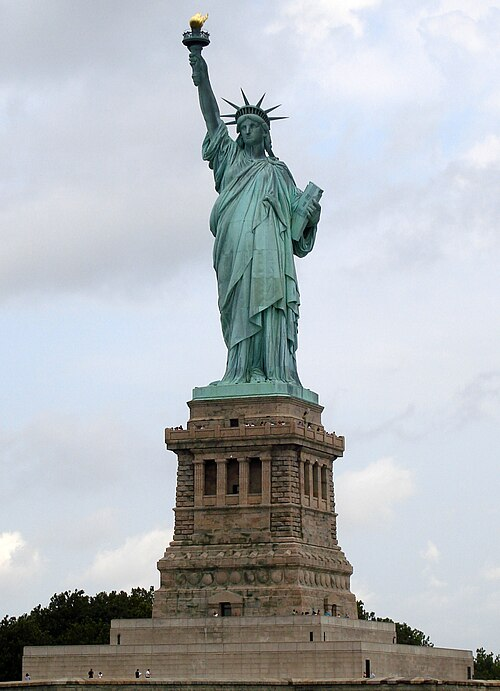
\includegraphics[width=0.32\linewidth]{images/book3/liberty.jpg}

{\small Una estatua de cobre de más de un siglo: su piel de fina chapa de cobre
se ha vuelto verde, cubierta por una pátina de sales básicas de cobre que protege el
metal subyacente. (Fotografía: Elcobbola, dominio público, Wikimedia Commons.)}
\end{omfigure}

\section{Protección}

La corrosión se combate separando el metal del agua y del oxígeno (pintura,
plástico, esmalte o una capa de otro metal), cambiando el medio
(eliminando el oxígeno, añadiendo inhibidores que se adsorben sobre el metal) o desplazando el
potencial del metal hasta su dominio de inmunidad.

\begin{definition}[Protección catódica]\label{def:b2:corrosion:protection}
La \emph{protección catódica}\index{proteccion catodica@protección catódica} rebaja el potencial de una
estructura metálica hasta que se detiene su oxidación, convirtiéndola en el cátodo de una pila.
La pila puede formarse con un \emph{ánodo de sacrificio}\index{anodo de sacrificio@ánodo de sacrificio},
un metal menos noble (cinc, magnesio, aleaciones de aluminio) conectado a la
estructura y consumido en su lugar, o accionarse con un generador, en la
\emph{protección por corriente impresa}\index{proteccion por corriente impresa@protección por corriente impresa}, siendo
entonces el ánodo un electrodo inerte enterrado en las proximidades.
\end{definition}

\begin{proposition}[Duración de un ánodo de sacrificio]\label{prop:b2:corrosion:anode-life}
Un \omterm{def:b2:corrosion:protection}{ánodo de sacrificio} de masa $m$ y masa molar $M$, oxidado con $n$ electrones
y un rendimiento $\eta$ (la fracción del metal que produce corriente útil,
corroyéndose el resto por sí solo), suministra una corriente $I$ durante un tiempo
\[
  t = \frac{\eta\,m\,nF}{M I} .
\]
\end{proposition}

\begin{proof}
La carga útil es $\eta\,(m/M)\,nF$; se divide por la corriente.
\end{proof}

\begin{omfigure}
\begin{tikzpicture}[font=\small, >={Stealth}]
  \fill[brown!20] (-4.2,-2.4) rectangle (4.2,0);
  \draw[thick] (-4.2,0) -- (4.2,0);
  \node[font=\scriptsize, anchor=south west] at (-4.2,0) {suelo};
  \fill[black!40] (-3.5,-1.6) rectangle (3.5,-1.2);
  \node[font=\scriptsize, white] at (0,-1.4) {tubería de acero (cátodo)};
  % sacrificial anode
  \fill[black!65] (-3.2,-2.3) rectangle (-2.2,-1.95);
  \node[font=\scriptsize, anchor=north] at (-2.7,-2.3) {ánodo de Mg};
  \draw[thick] (-2.7,-1.95) -- (-2.7,-1.6);
  \draw[->, omProp, thick] (-2.2,-2.12) -- (-1.4,-1.7);
  \node[font=\scriptsize, omProp, anchor=west] at (-1.9,-2.2) {corriente en el suelo};
  % impressed current
  \draw[thick, rounded corners] (1.8,0.4) rectangle (3.2,1.2);
  \node[font=\scriptsize] at (2.5,0.8) {rectificador};
  \fill[black!65] (3.4,-2.3) rectangle (3.9,-1.8);
  \node[font=\scriptsize, anchor=north] at (3.65,-2.3) {ánodo inerte};
  \draw[thick] (3.2,0.8) -- (3.65,0.8) -- (3.65,-1.8);
  \draw[thick] (1.8,0.8) -- (1.2,0.8) -- (1.2,-1.2);
  \node[font=\scriptsize, anchor=south] at (3.65,0.85) {$+$};
  \node[font=\scriptsize, anchor=south] at (1.2,0.85) {$-$};
  \node[font=\scriptsize, align=center] at (-2.7,0.8) {ánodo de sacrificio};
  \node[font=\scriptsize, align=center] at (2.5,1.55) {corriente impresa};
\end{tikzpicture}

{\small \omterm{def:b2:corrosion:protection}{Protección catódica} de una tubería enterrada, esquema. A la izquierda: un ánodo de
magnesio, conectado a la tubería, se corroe en su lugar. A la derecha: un rectificador hace pasar una
corriente desde un ánodo inerte a través del suelo hasta la tubería.}
\end{omfigure}

\begin{omfigure}
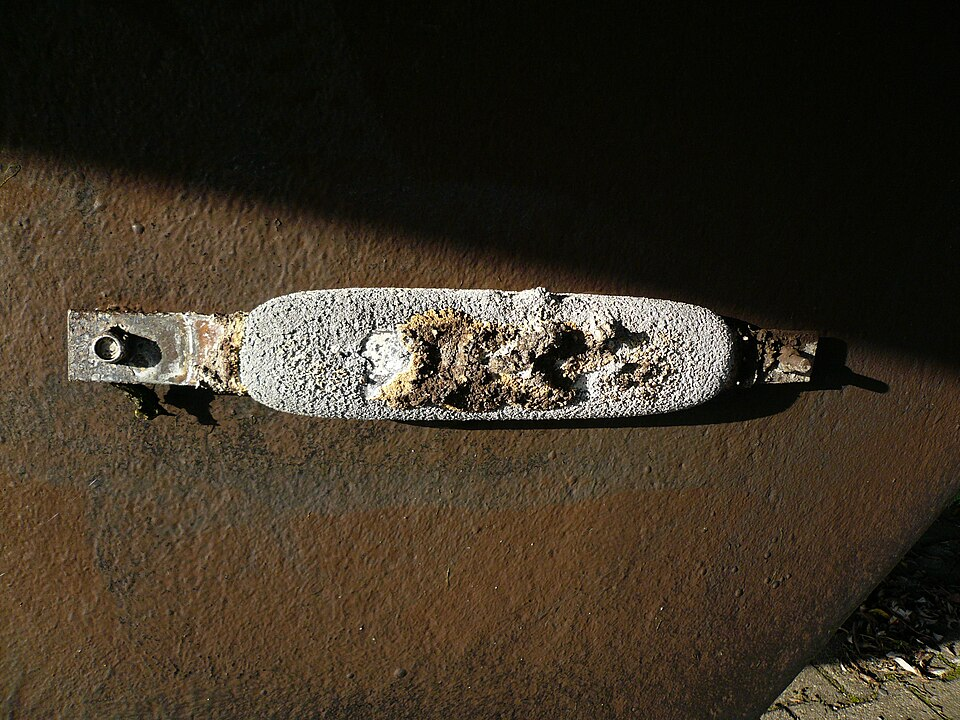
\includegraphics[width=0.5\linewidth]{images/book3/sacrificial-anode.jpg}

{\small Un \omterm{def:b2:corrosion:protection}{ánodo de sacrificio} de cinc atornillado al casco de acero de un barco, tras una
temporada en el agua: el cinc está carcomido, y el acero que lo rodea, intacto.
(Fotografía: Zwergelstern, CC BY-SA 3.0, Wikimedia Commons.)}
\end{omfigure}

\begin{omfigure}
\begin{tikzpicture}[font=\small, >={Stealth}, scale=1.35]
  \begin{scope}
    \fill[black!25] (0,0) rectangle (4,0.6);
    \fill[gray!55] (0,0.6) rectangle (1.7,0.8); \fill[gray!55] (2.3,0.6) rectangle (4,0.8);
    \fill[omDef!15] (0.8,0.8) .. controls (1.3,1.3) and (2.7,1.3) .. (3.2,0.8) -- (2.3,0.8) -- (2.3,0.6) -- (1.7,0.6) -- (1.7,0.8) -- cycle;
    \node[font=\scriptsize] at (2,-0.3) {acero galvanizado (capa de cinc)};
    \node[font=\scriptsize, align=center] at (2,1.6) {el cinc se corroe,\\ el acero queda protegido};
    \draw[->, omThm] (1.4,0.85) -- (1.8,0.65);
  \end{scope}
  \begin{scope}[xshift=5.5cm]
    \fill[black!25] (0,0) rectangle (4,0.6);
    \fill[gray!25] (0,0.6) rectangle (1.7,0.8); \fill[gray!25] (2.3,0.6) rectangle (4,0.8);
    \fill[omDef!15] (0.8,0.8) .. controls (1.3,1.3) and (2.7,1.3) .. (3.2,0.8) -- (2.3,0.8) -- (2.3,0.6) -- (1.7,0.6) -- (1.7,0.8) -- cycle;
    \fill[omProp] (1.75,0.6) rectangle (2.25,0.45);
    \node[font=\scriptsize] at (2,-0.3) {hojalata (capa de estaño)};
    \node[font=\scriptsize, align=center] at (2,1.6) {el acero se corroe en la raya,\\ deprisa (ánodo pequeño)};
  \end{scope}
\end{tikzpicture}

{\small Una raya a través de un recubrimiento metálico, esquema. El cinc, menos noble que el
hierro, se convierte en el ánodo y protege el acero expuesto, sea cual sea el tamaño de
la raya. El estaño, más noble que el hierro, se convierte en un gran cátodo alrededor de un pequeño
ánodo de acero, que se corroe más deprisa de lo que lo haría el acero desnudo.}
\end{omfigure}

\begin{method}[Elegir una protección]\label{met:b2:corrosion:choose-protection}
\begin{enumerate}
  \item Evítense los pares galvánicos: aíslense los metales distintos, o hágase que el menos
        noble sea el de mayor superficie.
  \item Recúbrase: un recubrimiento barrera (pintura, estaño) solo protege mientras está intacto; un
        recubrimiento de sacrificio (cinc) protege incluso rayado.
  \item Para una estructura en el suelo o en agua de mar, añádase \omterm{def:b2:corrosion:protection}{protección catódica}:
        \omterm{def:b2:corrosion:protection}{ánodos de sacrificio} para corrientes pequeñas o aguas conductoras,
        corriente impresa para estructuras largas o suelos resistivos.
  \item No se sobreproteja: un potencial demasiado bajo reduce el agua a hidrógeno en
        la estructura, lo que levanta los recubrimientos y puede fragilizar los aceros de alta
        resistencia.
\end{enumerate}
\end{method}

\section{Ejercicios}

\begin{exercise}[$\star$]\label{exo:b2:corrosion:1}
El cinc se corroe de forma uniforme bajo una densidad de corriente de \qty{2.0}{\micro A/cm^2}.
Calcúlese su pérdida de espesor por año ($\rho = \qty{7.13}{g/cm^3}$).
\end{exercise}

\begin{exercise}[$\star$]\label{exo:b2:corrosion:2}
Unos pernos de acero sujetan chapas de cobre en un tejado. ¿Qué metal se corroe? La misma pregunta
para clavos de cinc en chapas de acero.
\end{exercise}

\begin{exercise}[$\star$]\label{exo:b2:corrosion:3}
Dos chapas de acero se sujetan con un perno y se dejan en agua de mar. ¿Dónde se
concentra la corrosión, y por qué?
\end{exercise}

\begin{exercise}[$\star$]\label{exo:b2:corrosion:4}
Un cubo galvanizado y una lata de hojalata se rayan hasta el acero. ¿Cuál
se oxida en la raya?
\end{exercise}

\begin{exercise}[$\star\star$]\label{exo:b2:corrosion:5}
En el diagrama de Evans del hierro en agua aireada, explíquese qué les ocurre al
potencial y a la \omterm{def:b2:corrosion:uniform}{corriente de corrosión} cuando se agita el agua y luego cuando se
la desprovee de oxígeno.
\end{exercise}

\begin{exercise}[$\star\star$]\label{exo:b2:corrosion:6}
Un ánodo de cinc de \qty{5.0}{kg} protege el casco de un barco con una corriente de
\qty{0.10}{A}, con un rendimiento del 90~\% (datos del ejercicio). ¿Cuánto tiempo
dura?
\end{exercise}

\begin{exercise}[$\star\star$]\label{exo:b2:corrosion:7}
Calcúlense la carga, en amperios hora por kilogramo, que suministran los ánodos de cinc, magnesio
y aluminio con un rendimiento del 100~\%, y los potenciales estándar de
sus pares a partir de $\Delta_f G^\circ$ (\ce{Zn^2+} $-147.06$, \ce{Mg^2+} $-454.8$,
\ce{Al^3+} $-485$ \unit{kJ/mol}). ¿Por qué se prefiere el magnesio en suelos secos?
\end{exercise}

\begin{exercise}[$\star\star$]\label{exo:b2:corrosion:8}
Una tubería enterrada necesita \qty{2.0}{A} de corriente de protección. El lecho anódico del
ánodo inerte tiene una resistencia de \qty{4.0}{\ohm} respecto del suelo y la celda necesita
\qty{1.5}{V} adicionales (datos del ejercicio). Calcúlense la tensión del rectificador y la
energía eléctrica por año.
\end{exercise}

\begin{exercise}[$\star\star$]\label{exo:b2:corrosion:9}
Un pilote de acero está en el mar. Explíquese por qué se corroe sobre todo un poco por debajo de
la línea de flotación, y no en la propia línea de flotación.
\end{exercise}

\begin{exercise}[$\star\star\star$]\label{exo:b2:corrosion:10}
Explíquese, con la curva pasiva, por qué el acero inoxidable resiste el agua aireada pero
puede picarse en agua de mar, y por qué una picadura, una vez iniciada, crece en profundidad y no
en anchura.
\end{exercise}

\begin{exercise}[$\star\star\star$]\label{exo:b2:corrosion:11}
Un racor de cobre está enroscado en una tubería de acero por la que circula agua aireada. La
densidad de \omterm{def:b2:current-potential-curves:limiting-current}{corriente límite} del oxígeno es de \qty{5}{\micro A/cm^2} sobre toda superficie mojada; el
cobre ofrece \qty{20}{cm^2} y el acero cerca de la junta \qty{2}{cm^2}
(datos del ejercicio). Estímense la \omterm{def:b2:corrosion:uniform}{corriente de corrosión} del acero y su pérdida de
espesor por año cerca de la junta.
\end{exercise}

\begin{exercise}[$\star\star\star$]\label{exo:b2:corrosion:12}
Con el diagrama E--pH del hierro y las curvas del agua, explíquese por qué el
potencial de una estructura de acero protegida debe mantenerse por debajo de unos
\qty{-0.6}{V}, pero no muy por debajo de \qty{-1}{V}, en agua neutra.
\end{exercise}

\section{Problema: proteger un oleoducto}

\begin{problem}[{Problema de fin de semana --- la corrosión de una tubería de acero desnuda en un
suelo húmedo, la elección de un metal de sacrificio, el magnesio necesario para veinte años
y la alternativa de la corriente impresa}]
\label{pb:b2:corrosion:1}
Un oleoducto de acero de \qty{10.0}{km} de longitud y \qty{0.30}{m} de diámetro está enterrado en
suelo húmedo. Datos: hierro, $M = \qty{55.845}{g/mol}$, $\rho = \qty{7.87}{g/cm^3}$;
magnesio, $M = \qty{24.305}{g/mol}$; $\Delta_f G^\circ$ (\unit{kJ/mol}): \ce{Fe^2+}
$-78.90$, \ce{Zn^2+} $-147.06$, \ce{Mg^2+} $-454.8$, \ce{Al^3+} $-485$. Datos del
ejercicio: densidad de \omterm{def:b2:corrosion:uniform}{corriente de corrosión} del acero desnudo en este suelo \qty{10}{\micro
A/cm^2}; densidad de corriente de diseño para la protección del acero desnudo
\qty{20}{mA/m^2}; el recubrimiento deja desnudo el 1.0~\% de la superficie; ánodos de magnesio
de \qty{15}{kg}, rendimiento 50~\%; resistencia del lecho anódico para la corriente impresa
\qty{5.0}{\ohm}.
% ledger: aw:Fe, rho:Fe, aw:Mg, dfg:Fe2+_ao, dfg:Zn2+_ao, dfg:Mg2+_ao, dfg:Al3+_ao, const:F

\medskip
\noindent\textbf{Parte I --- La tubería desnuda.}
\begin{enumerate}
  \item Escríbanse las reacciones anódica y catódica sobre la tubería.
  \item ¿Por qué fija el aporte de oxígeno la \omterm{def:b2:corrosion:uniform}{corriente de corrosión}?
  \item Calcúlese la masa de hierro perdida por metro cuadrado y por año.
  \item Calcúlese la pérdida de espesor de la pared por año.
  \item ¿Cuánto tardaría la tubería desnuda en perder la mitad de una pared de \qty{8}{mm}?
  \item ¿Por qué la tubería real falla antes, en unos pocos puntos?
\end{enumerate}

\medskip
\noindent\textbf{Parte II --- El metal del ánodo.}
\begin{enumerate}[resume]
  \item Calcúlense los potenciales estándar de los pares del hierro, el cinc, el magnesio
        y el aluminio.
  \item ¿Qué metales pueden proteger el hierro como \omterm{def:b2:corrosion:protection}{ánodos de sacrificio}?
  \item ¿Por qué se usa poco el aluminio en los suelos?
  \item ¿Por qué se prefiere el magnesio al cinc en un suelo de resistividad elevada?
  \item Calcúlese la masa de magnesio consumida por amperio y por año.
\end{enumerate}

\medskip
\noindent\textbf{Parte III --- Diseño.}
\begin{enumerate}[resume]
  \item Calcúlese la superficie exterior de la tubería.
  \item Calcúlese la superficie desnuda que deja el recubrimiento.
  \item Calcúlese la corriente de protección.
  \item Calcúlese la carga necesaria para veinte años.
  \item Calcúlese la masa de magnesio necesaria.
  \item ¿Cuántos ánodos hacen falta?
  \item ¿Por qué se reparten a lo largo de la tubería en lugar de enterrarlos en un
        solo punto?
\end{enumerate}

\medskip
\noindent\textbf{Parte IV --- Corriente impresa.}
\begin{enumerate}[resume]
  \item Descríbase la alternativa de la corriente impresa.
  \item Estímese la tensión del rectificador a partir de la resistencia del lecho anódico,
        añadiendo \qty{1.5}{V} para los electrodos.
  \item Calcúlese la energía eléctrica empleada por año.
  \item ¿Qué falla si la tubería está sobreprotegida?
  \item ¿Por debajo de qué potencial es inmune el hierro en agua neutra, tomando una
        concentración de hierro(II) de \qty{1e-6}{mol/L}?
  \item Indíquese la masa de ánodos de magnesio necesaria para veinte años.
\end{enumerate}
\end{problem}
